
\subsubsection{10.10.14}

\begin{enumerate}
	\item Время начала и окончания собрания:
	18:30 - 21:40
	\item Цели собрания:
	\begin{enumerate}
	  \item Выбрать оптимальный диаметр поперечных балок для подъемника.
	  
	  \item Распилить алюминиевый профиль на сегменты нужной длины, просверлить в них нужные отверстия и установить их между направляющими вместо прослойки из оригинальной тетриксовской детали.
	  
    \end{enumerate}
	\item Проделанная работа:
	\begin{enumerate}
	  \item Был приобретен ремень для раздвигания подъемника.
	  
	  \begin{figure}[H]
	  	\begin{minipage}[h]{0.2\linewidth}
	  		\center  
	  	\end{minipage}
	  	\begin{minipage}[h]{0.6\linewidth}
	  		\center{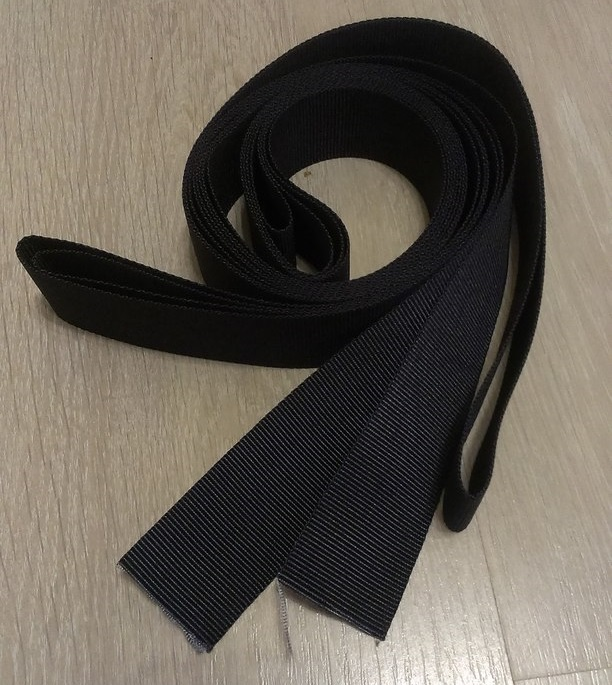
\includegraphics[scale=0.3]{days/10.10.14/images/01}}
	  		\caption{Ремень}
	  	\end{minipage}
	  \end{figure}
      
      \item  Для создания креплений для поперечных балок была приобретена алюминиевая полоса размерами 200 см х 5 см х 0,2 см.
      
      \item В качестве поперечных балок в наборе TETRIX были доступны цилиндрические валы диаметром 15 мм и оси для колес диаметром 5 мм. Предпочтение было отдано последним по причине их большей компактности.
       
      \item Поскольку оси меньшего диаметра имели срезанный край для закрепления втулок колес, они оказывали большое сопротивление движению ремня из-за трения. Тогда было решено насадить на ось свободные (без креплений) втулки. Предварительные испытания продемонстрировали полную состоятельность данной идеи.
        
      \item После этого было решено приступить к действиям:
      \begin{enumerate}
      	\item Направляющие подъемника были предварительно разобраны.
      	
      	\item  Алюминиевая полоса была распилена на 6 сегментов: 2 по 30 см и 4 по 35 см.
      	
      	\item При сверлении полученных деталей возникли трудности, поскольку все сверла оказались сточенными. К следующему занятию было решено купить новые сверла.
      	
      	\begin{figure}[H]
      		\begin{minipage}[h]{0.2\linewidth}
      			\center  
      		\end{minipage}
      		\begin{minipage}[h]{0.6\linewidth}
      			\center{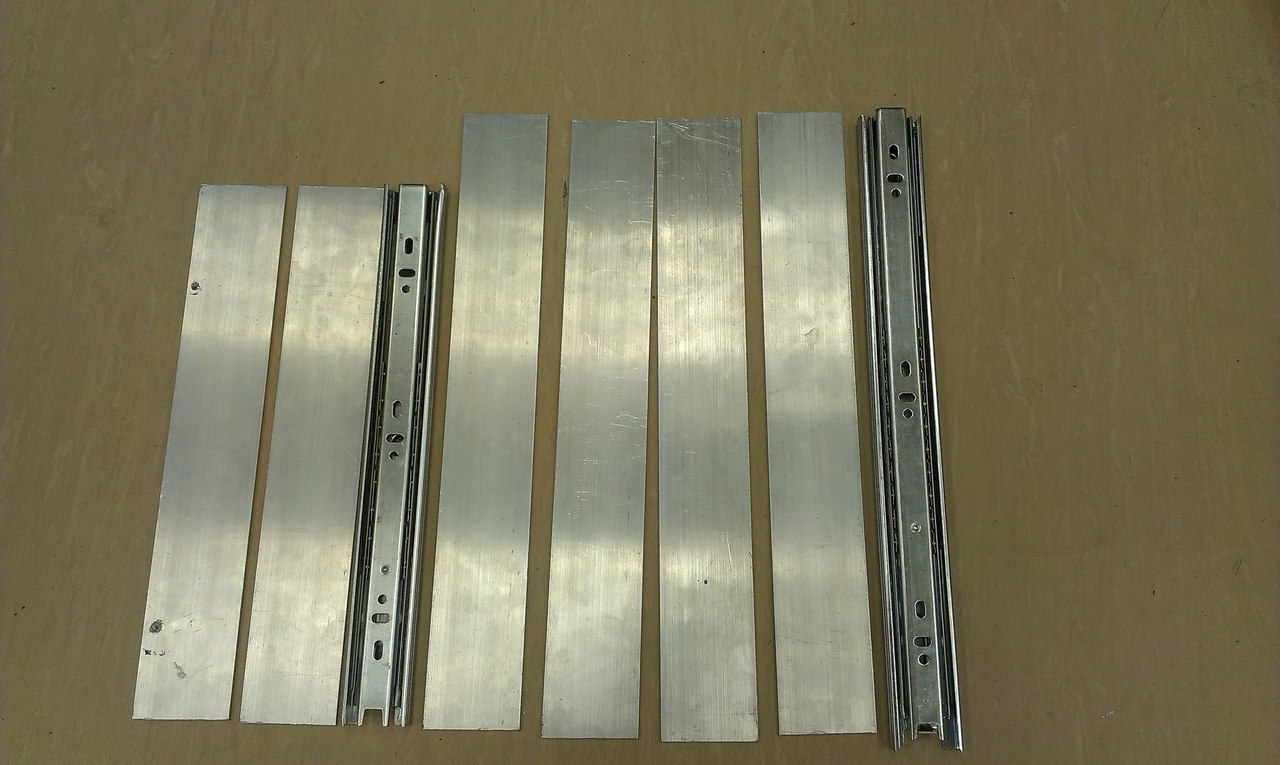
\includegraphics[scale=0.2]{days/10.10.14/images/02}}
      			\caption{Алюминиевая полоса была распилена на 6 сегментов}
      		\end{minipage}
      	\end{figure}
      	
      \end{enumerate}
      
    \end{enumerate}
    
	\item Итоги собрания: 
	\begin{enumerate}
	  \item Выбраны балки для подъемника.
	  
	  \item Балка распилена на сегменты нужной длины.
	  
	  \item Просверлить отверстия не удалось.
	   
    \end{enumerate}
    
	\item Задачи для последующих собраний:
	\begin{enumerate}
	  \item Купить новые сверла по металлу.
	  
    \end{enumerate}     
\end{enumerate}
\fillpage
